\documentclass[a4paper,12pt]{article} % тип документа
\usepackage[margin=1in]{geometry} % Поля

%  Русский язык
\usepackage[warn]{mathtext}
\usepackage[T2A]{fontenc}			% кодировка
\usepackage[utf8]{inputenc}			% кодировка исходного текста
\usepackage[english,russian]{babel}	% локализация и переносы
% Математика
\usepackage{amsmath,amsfonts,amssymb,amsthm,mathtools} 
\usepackage{wasysym}
%%%
\usepackage{graphicx}

\usepackage{tabularx}

\usepackage{gensymb} % знак градуса
\usepackage{enumitem} % изменить список enumerate
\usepackage{placeins} % \FloatBarrier

\renewcommand{\thesection}{\Roman{section}} 
\renewcommand{\thesubsection}{\roman{subsection}}


\begin{document}

\newcolumntype{Y}{>{\centering\arraybackslash}X} %new tabularx


%титул
\hrule 	
\medskip
\begin{raggedright}
{\large \textbf{Вопрос по выбору для экзамена по общей физике по разделу <<Электричество и магнетизм>>}}
\\
\medskip
{\Large Способы определения размера элементарного электрического заряда. Опыт Милликена.} 
\\
\medskip
{\large Карташов Констанин Б04-005}
\medskip
\hrule
\medskip
\end{raggedright}


\section{Анотация}

\paragraph{} В данном вопросе по выбору дано современное определение элементарному электрическому заряду, рассмотрено несколько способов нахождение этой величины, проведён опыт Миллекена где показан способ нахождения элементарного заряда и оценка погрешности. 

\paragraph{Оборудование:}
\begin{itemize}
\renewcommand{\labelitemi}{$\triangleright$}
\itemsep0em
\item итем
\end{itemize}


\medskip\hrule\medskip

\section{Определение и нахождение элементарного электрического заряда}

\paragraph{Современное фиксированное значение.} Элементарный электрический заряд -- фундаментальная физическая постоянная, минимальная порция (квант) электрического заряда, наблюдающегося в природе у свободных долгоживущих частиц. Согласно изменениям определений основных единиц СИ равен точно $1,602 \, 176 \, 634 \cdot 10^{-19}$ Кл в Международной системе единиц (СИ) (В системе СГСЭ он равен $4,803\,204\,25\,(10) \cdot 10^{-10}$ Фр).

\paragraph{Отношение через другие физические постоянные.} Элементарный заряд можно выразить через отношение:

\[ e^2 = \frac{2h\alpha}{\mu_0 c} = 2 h \alpha \varepsilon_0 c,
\]

\noindent где $h$ -- постоянная Планка, $\alpha$ -- постоянная тонкой структуры, $\mu_0$ -- магнитная постоянная,  $\varepsilon_0$ -- электрическая постоянная, $c$ -- скорость света в вакууме. До 2019 $\varepsilon_0$ было фиксированным значением. Сейчас в этой формуле зафиксированы все постоянные кроме $\alpha$ и $\varepsilon_0$.

\paragraph{Отношение постоянной Фарадея и числа Авогадро.} Число Авогадро и постоянную Фарадея можно вычислить экспериментальным способом, из чего можно получить значение для элементарного заряда из отношения $q = F / N_A$. Точность этого способа ограниченная точностью измерения постоянной $F$, относительная погрешность которой в лучшем случае равна $\varepsilon = 1.6 \cdot 10^{-3}$.

\paragraph{Дробовой шум.} Дробовой шум вызван дискретностью электрического заряда. Поэтому при анализе дробового шума можно получить значение для элементарного заряда с точностью до нескольких процентов. Формула Шоттки для спектральной плотности дробового шума:

\[ \frac{\langle \Delta I^2 \rangle}{\Delta \nu} = 2e A \langle I \rangle,\; A \approx 1.
\]

\paragraph{Опыт Милликена.} Опыт Милликена или эксперимент с каплей масла -- важный эксперимент по определению электрического заряда электрона. Он назван в честь американского физика Роберта Эндрюса Милликена, который провёл этот опыт совместно с Харви Флетчером в 1909 году. Милликен усовершенствовал его в 1913 году и в 1923 году получил Нобелевскую премию по физике. 

Опыт, по сути, состоял в создании капель масла с помощью распылителя и наблюдении за их поведением в электрическом поле. Некоторые из капель были электрически заряжены в результате захвата ионов после облучения воздуха рентгеновским излучением, и, задав соответствующее значение электрического поля, можно было управлять вертикальным движением капель. Измеряя напряжённость электрического поля, необходимого для противодействия силе тяжести и, зная массу капель, которую можно вычислить, измеряя скорость их свободного падения в воздухе, Миллигенри заметил, что значения электрических зарядов капель всегда были целыми числами кратными фиксированной величине, которая стала отождествляться с элементарным зарядом. Полученное значение составило $e = -1,5924(17) \cdot 10^{-19}$ Кл, всего на $0,62 \%$ ниже принятого в настоящее время значения. (Схема установки на рис. \ref{millakan})


\begin{figure}[h]
\centering
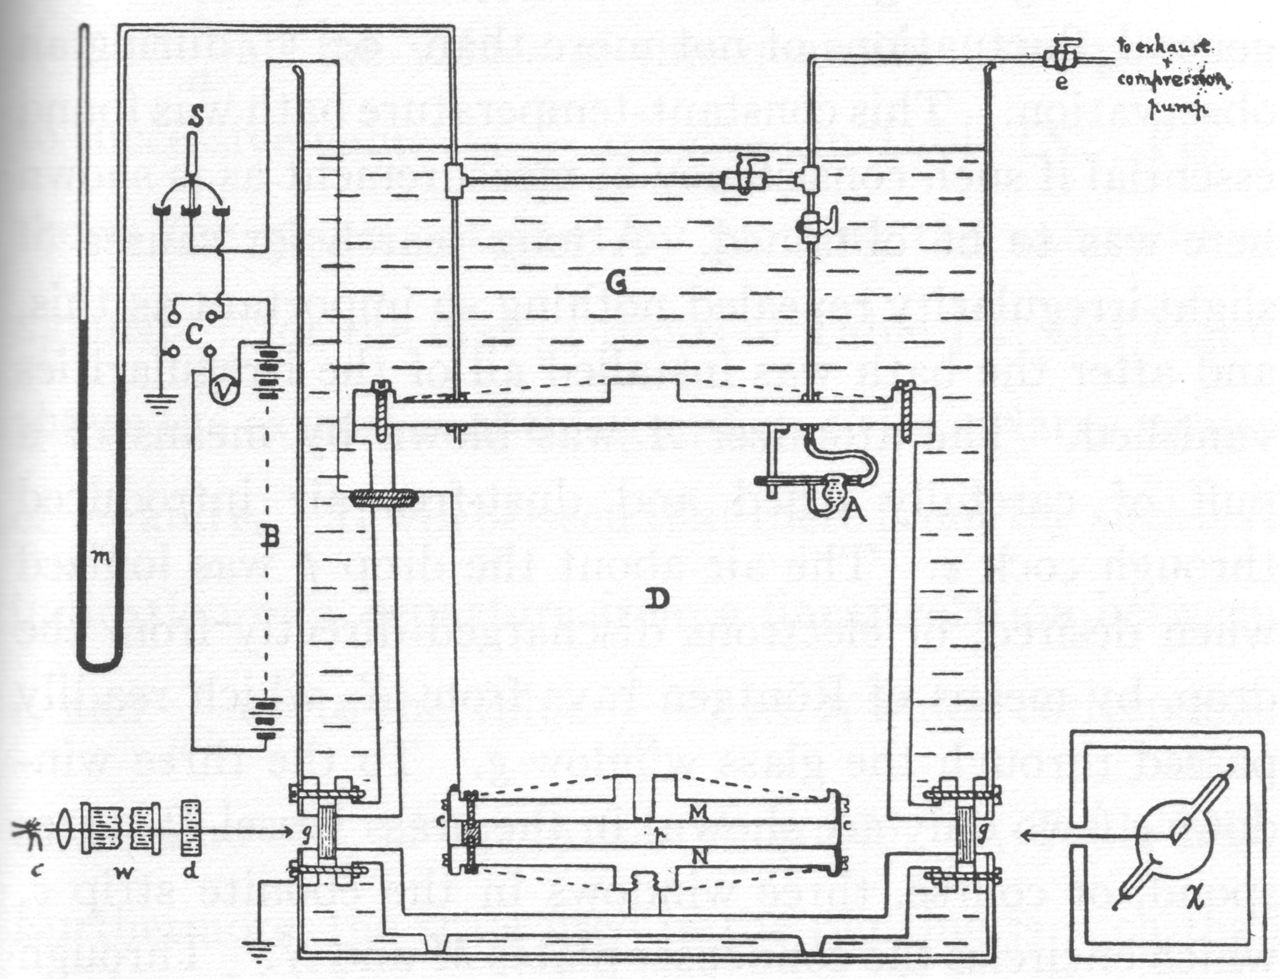
\includegraphics[width=0.7\textwidth]{millakin.jpg}
\caption{Схема установки используемой Р.А.Миллекеном в 1917 году}
\label{millakan}
\end{figure}

\medskip\hrule\medskip

\section{Проведение опыта Миллекена}

\paragraph{Уравнение движения капли.} Рассмотрим свободное падение капли в воздухе. Второй закон Ньютона для неё имеет вид:

\begin{equation}
m\frac{dv}{dt} = mg - F_\text{тр}, \label{2new}
\end{equation} 

\noindent где $m$ -- масса капли, $v$ -- её скорость, $g$ -- ускорение свободного падения, $F_\text{тр}$ -- сила вязкого трения в воздухе. Сила вязкого трения определяется формулой Стокса:

\begin{equation}
F_\text{тр} = 6 \pi \eta r v = kv, \label{stocks}
\end{equation}

\noindent где $r$ -- радиус капли, $\eta$ -- коэффициент вязкости воздуха.

Подставляя (\ref{stocks}) в (\ref{2new}) и интегрируя при нулевой начальной скорости, получим:

\begin{equation}
v = v_\infty \left( 1 - e^{- \frac{kt}{m}} \right). \label{vinf}
\end{equation}

\noindent Здесь $v_\infty$ -- предельная скорость падения, равная:

\begin{equation}
v_\infty = \frac{mg}{k} = \frac{\frac{4}{3}\pi\rho r^3 g}{6 \pi \eta r} = \frac{2}{9} \frac{\rho}{\eta} g r^2, \label{vinf2}
\end{equation}

\noindent где $rho$ -- плотность масла.

Из (\ref{vinf}) найдём характерное время установления предельной скорости:

\begin{equation}
\tau = \frac{m}{k} = \frac{v_\infty}{g} = \frac{2}{9} \frac{\rho}{eta} r^2.
\end{equation}

\noindent Из этого видим, что для мелких капель время установления много меньше любых других процессов. Поэтому скорость можно считать установившейся всегда, то есть движение равномерно и имеет скорость $v_\infty$.

Из (\ref{vinf2}) найдём радиус капли подставив $h = v_\infty t$:

\begin{equation}
r = \sqrt{\frac{9\eta h}{2 \rho g t}}. \label{radius}
\end{equation}

Теперь рассмотрим движение капли в электрическом поле с напряжённостью $E = U/l$, где $l$ -- расстояние между пластинами, $U$ -- разностью потенциала между ними. Для поднимающейся капли уравнение движения будет иметь вид:

\begin{equation}
m \frac{dv}{dq} = \frac{qU}{l} - mg - kv, \label{new2}
\end{equation}

\noindent где $q$ -- заряд капли. При этом характерное время установления не изменяется. И новая скорость получается равной:

\begin{equation}
v_\infty' = \frac{qU}{kl} - v_\infty. \label{vinf3}
\end{equation}

Пусть $t' = h / v_\infty'$ -- время подъёма капли на начальную высоту. Используя формулы (\ref{stocks}), (\ref{radius}) и (\ref{vinf3}), получим окончательную расчётную формулу:

\begin{equation}
q = 9 \pi \frac{l}{U} \sqrt{\frac{2}{\rho g}} (\eta h)^{\frac{3}{2}} \frac{t + t'}{t^\frac{3}{2} t'}. \label{final}
\end{equation}

Постоянные:

\begin{itemize}
\item $g = 9.8155$ м/с$^2$ (в Москве)
\item $\eta = 1.85 \cdot 10^{-5}$ Па $\cdot$ с
\end{itemize}

\paragraph{Экспериментальная установка.} Схема установки приведена на рис. \ref{setup}. Масло разбрызгивается пульверизатором. Капли масла попадают в конденсатор $C$ через небольшое отверстие в верхней пластине. При этом часть из них вследствие трения об воздух приобретают случайный по величине и знаку заряд.

Напряжение на пластины подаётся от регулируемого выпрямитель и измеряется вольтметром V. Ключ K позволяется менять направления поля в конденсаторе. При размыкании ключа конденсатор разряжается через дополнительное сопротивление $R \approx 10$ МОм.

Картинку видную через окуляр микроскопа можно увидеть на рис. \ref{drops}.


Постоянные установки:
\begin{itemize}
\item $\rho = 0.898 \; \text{г/см}^3 = 898 \; \text{кг/м}^3$
\item $d = 0.725 \; \text{см} = 7.25 \cdot 10^{-4} \; \text{м}$
\end{itemize}

\begin{figure}[h]
\centering
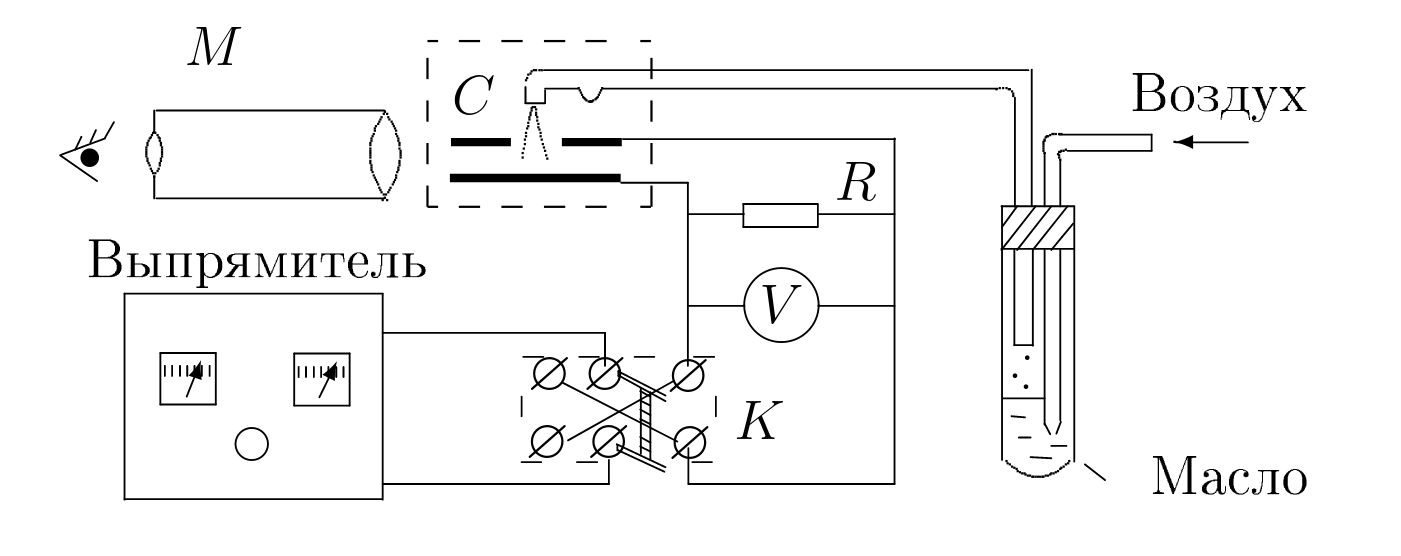
\includegraphics[width=0.7\textwidth]{setup.png}
\caption{Схема экспериментальной установки}
\label{setup}
\end{figure}

\begin{figure}
\centering
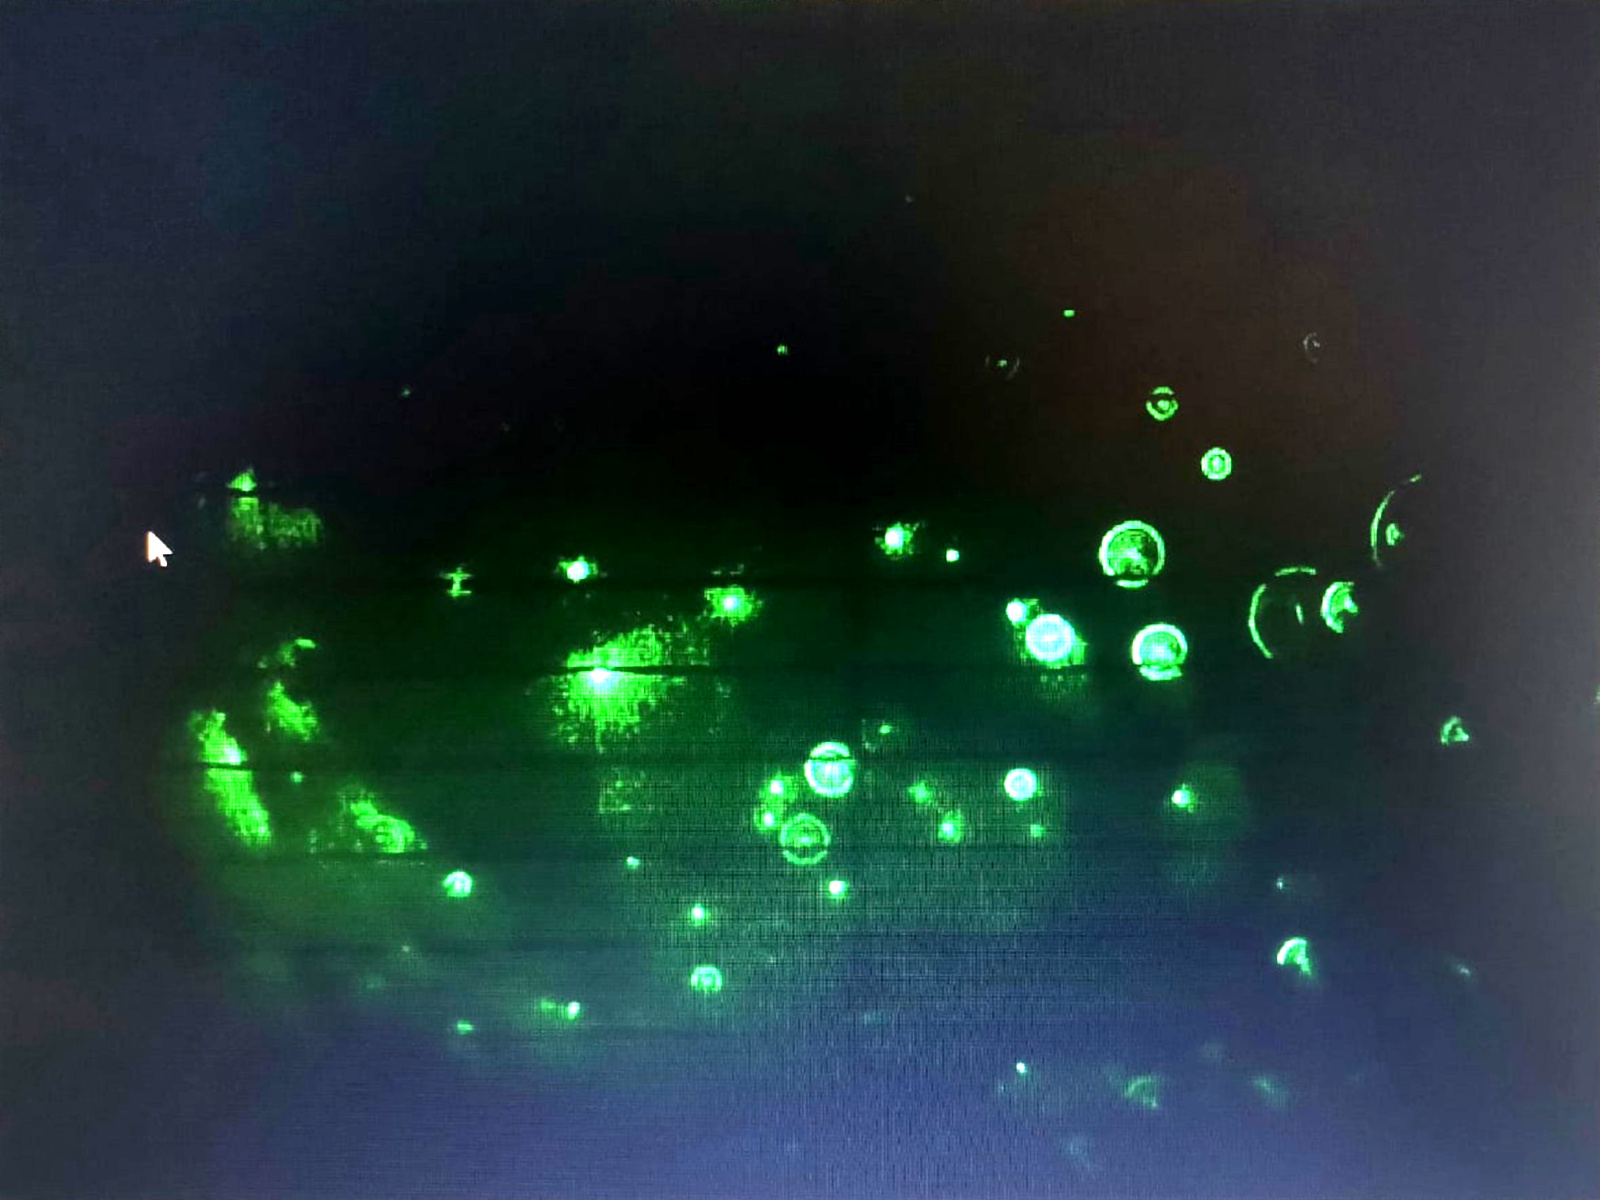
\includegraphics[width=0.7\textwidth]{drops.jpg}
\caption{Картинка капель освещённых лазером}
\label{drops}
\end{figure}

\paragraph{Проведённые измерения.} Мы измерили время падения и возвращения для 7-ми капель и соответствующие напряжения на конденсаторе (табл. 1).

\begin{table}[h]
\centering
\begin{tabular}{|ll|ll|ll|ll|ll|ll|ll|}
\hline
\multicolumn{2}{|l|}{$U = 465$ В} & \multicolumn{2}{l|}{$U = 385$ В} & \multicolumn{2}{l|}{$U = 435$ В} & \multicolumn{2}{l|}{$U = 425$ В} & \multicolumn{2}{l|}{$U = 415$ В} & \multicolumn{2}{l|}{$U = 485$ В} & \multicolumn{2}{l|}{$U = 485$ В} \\ \hline
\multicolumn{1}{|l|}{$t$, с} & $t'$, с & \multicolumn{1}{l|}{$t$, с} & $t'$, с & \multicolumn{1}{l|}{$t$, с} & $t'$, с & \multicolumn{1}{l|}{$t$, с} & $t'$, с & \multicolumn{1}{l|}{$t$, с} & $t'$, с & \multicolumn{1}{l|}{$t$, с} & $t'$, с & \multicolumn{1}{l|}{$t$, с} & $t'$, с \\ \hline
\multicolumn{1}{|l|}{39.5} & 16.9 & \multicolumn{1}{l|}{19.8} & 13 & \multicolumn{1}{l|}{54.8} & 14.6 & \multicolumn{1}{l|}{10.2} & 23.1 & \multicolumn{1}{l|}{29.1} & 10.5 & \multicolumn{1}{l|}{20.1} & 16.5 & \multicolumn{1}{l|}{25.5} & 12 \\ \hline
\multicolumn{1}{|l|}{40.4} & 18.1 & \multicolumn{1}{l|}{18.7} & 12.6 & \multicolumn{1}{l|}{53.2} & 14.4 & \multicolumn{1}{l|}{10.4} & 22.8 & \multicolumn{1}{l|}{28.6} & 11.1 & \multicolumn{1}{l|}{19.5} & 17.4 & \multicolumn{1}{l|}{25.6} & 11.7 \\ \hline
\multicolumn{1}{|l|}{43.5} & 17.6 & \multicolumn{1}{l|}{18.5} & 13.3 & \multicolumn{1}{l|}{49.2} & 15.2 & \multicolumn{1}{l|}{9.8} & 23.1 & \multicolumn{1}{l|}{32} & 11 & \multicolumn{1}{l|}{20.8} & 16.5 & \multicolumn{1}{l|}{24.2} & 12 \\ \hline
\multicolumn{1}{|l|}{38.9} & 18.2 & \multicolumn{1}{l|}{18.2} & 13.7 & \multicolumn{1}{l|}{59.8} & 14.8 & \multicolumn{1}{l|}{--} & -- & \multicolumn{1}{l|}{38.7} & 11.1 & \multicolumn{1}{l|}{21.4} & 16.6 & \multicolumn{1}{l|}{--} & -- \\ \hline
\multicolumn{1}{|l|}{40.1} & 17.1 & \multicolumn{1}{l|}{--} & -- & \multicolumn{1}{l|}{--} & -- & \multicolumn{1}{l|}{--} & -- & \multicolumn{1}{l|}{30} & 11.3 & \multicolumn{1}{l|}{20} & 16.9 & \multicolumn{1}{l|}{--} & -- \\ \hline
\multicolumn{1}{|l|}{39.2} & 18.3 & \multicolumn{1}{l|}{--} & -- & \multicolumn{1}{l|}{--} & -- & \multicolumn{1}{l|}{--} & -- & \multicolumn{1}{l|}{--} & -- & \multicolumn{1}{l|}{--} & -- & \multicolumn{1}{l|}{--} & -- \\ \hline
\end{tabular}
\caption{Измерения для 7-ми капель}
\label{data}
\end{table}

Подставив данные из табл. \ref{data} в формулу (\ref{final}) получим заряд и среднее квадратичное случайной погрешности. Дальше пронаблюдаем закономерности в размерах значений, из чего найдём $n$ -- кратность заряда на капельке. Данные занесём в табл. \ref{charges}.

\begin{table}[h]
\centering
\begin{tabular}{|c|c|c|c|}
\hline 
$q$, Кл $\cdot 10^{-19}$ & $\sigma_q$, Кл $\cdot 10^{-19}$ & $\varepsilon_q^\text{сл}$ & n \\ 
\hline 
2.15 & 0.09 & 0.04 & 2 \\ 
\hline 
6.04 & 0.23 & 0.04 & 6 \\ 
\hline 
2.1 & 0.11 & 0.05 & 2 \\ 
\hline 
8.19 & 0.32 & 0.04 & 8 \\ 
\hline 
4.3 & 0.2 & 0.05 & 4 \\ 
\hline 
3.87 & 0.13 & 0.03 & 3 \\ 
\hline 
3.97 & 0.12 & 0.03 & 3 \\ 
\hline 
\end{tabular} 
\caption{Полученные заряды капель}
\label{charges}
\end{table}

Оценим экспериментальную погрешность исходя из соображений, что $t ~ t'$, и $\Delta U \approx 0.01$, $\Delta t \approx 0.2$ по формуле:

\[
\varepsilon_q ~ \sqrt{\left( \frac{\Delta U}{U} \right)^2 + \left( \frac{\Delta t}{t' + t} \right)^2}
\]

\noindent Для значений из таблицы \ref{data} найдём:

\begin{center}
\begin{tabular}{|c|c|c|c|c|c|c|c|}
\hline 
$\varepsilon_q^\text{пр}$ & 0.02 & 0.03 & 0.02 & 0.03 & 0.03 & 0.03 & 0.02 \\ 
\hline 
\end{tabular} 
\end{center}

Значения для элементарного заряда найдём построив график зависимости $q(n)$ для полученных данных. По методу наименьших квадратов проведём прямую, и в точке $n = 1$ найдём значение для элементарного заряда (рис. \ref{plot1}).

\begin{figure}[h]
\centering
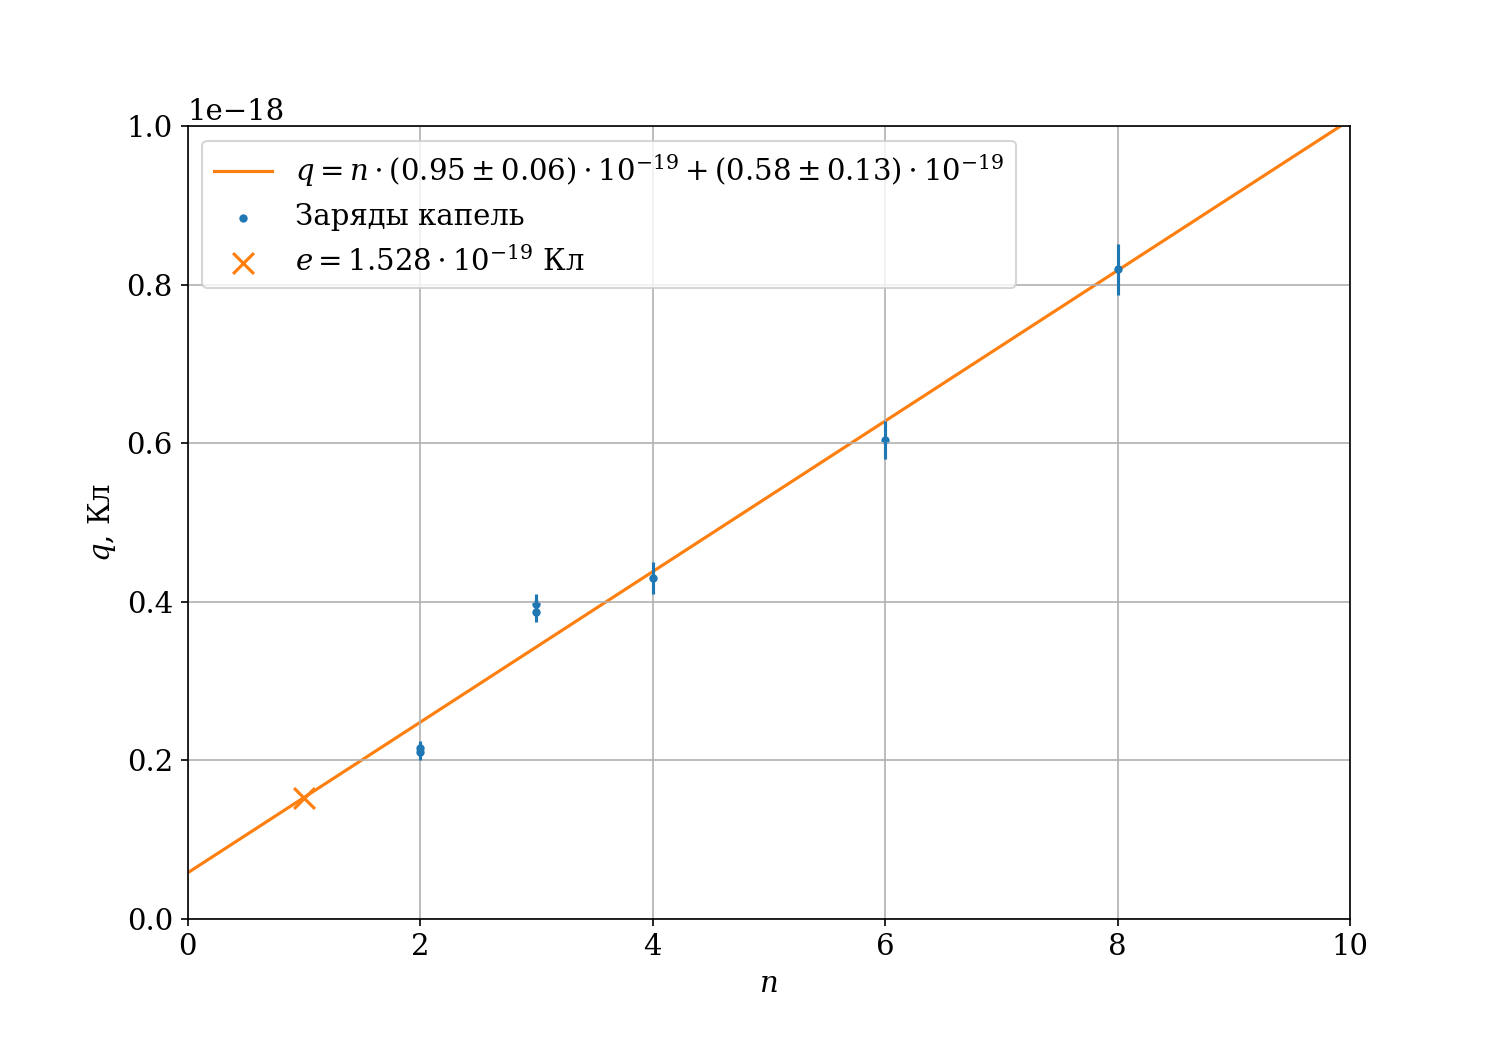
\includegraphics[width=\textwidth]{plot1.png}
\caption{Зависимость полученных зарядов от $n$}
\label{plot1}
\end{figure} 

Из графика получаем $e = 1.528 \cdot 10^{-19}$ Кл, а также $\varepsilon_e^\text{сл} = 0.06$. Найдём общую относительную погрешность по формуле: $\varepsilon_e = \sqrt{(\varepsilon_q^\text{сл})^2 + (\varepsilon_q^\text{пр})^2 + (\varepsilon_e^\text{сл})^2}$. Тогда $\Delta e = \varepsilon_e \cdot e = 1.528 \cdot 10^{-19} \cdot \sqrt{0.05^2 + 0.03^2 + 0.06^2} = 0.128 \cdot 10^{-19}$. Получаем $e = (1.53 \pm 0.13) \cdot 10^{-19}$ Кл. Реальное значение элементарного заряда действительно лежит в этих пределах.


\paragraph{Итог.} Получен заряд $e = (1.53 \pm 0.13) \cdot 10^{-19}$ Кл, чем мы продемонстрировали эффективность опыта Миллекена. Видно, что при увеличении количества измерений легко получить более высокую точность.


\medskip\hrule\medskip

\end{document}
